\documentclass[border=3pt,tikz]{standalone}
\usetikzlibrary{angles,quotes}
\usetikzlibrary{calc}% needed for \MarkRightAngle
\newcommand{\MarkRightAngle}[4][.25cm]% #1=size (optional), #2-#4 three points: \angle #2#3#4
{\coordinate (tempa) at ($(#3)!#1!(#2)$);
    \coordinate (tempb) at ($(#3)!#1!(#4)$);
    \coordinate (tempc) at ($(tempa)!0.5!(tempb)$);%midpoint
    \draw (tempa) -- ($(#3)!2!(tempc)$) -- (tempb);
}

\begin{document}

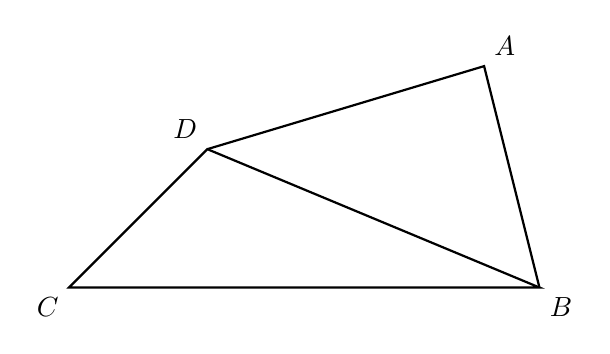
\begin{tikzpicture}[x=10,y=10, thick]
  \coordinate (C)  at (0,0);
  \coordinate (B)  at (17,0);
  \coordinate (D)  at (5,5);
  \coordinate (A)  at (15,8);
  \draw (C) node[below left] {$C$} -- (B) node[below right] {$B$} -- (D) node[above left] {$D$} -- cycle; 
  \draw (D) -- (A) node[above right] {$A$} -- (B);
\end{tikzpicture}

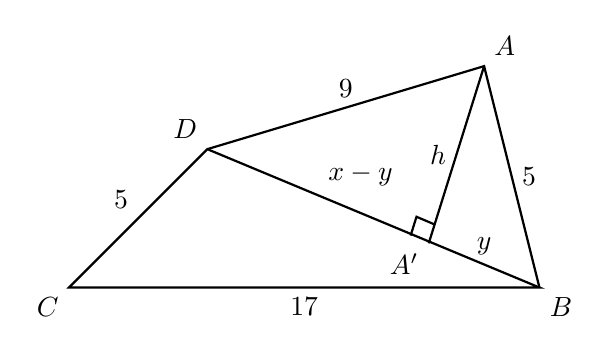
\begin{tikzpicture}[x=10,y=10, thick]
  \coordinate (C)  at (0,0);
  \coordinate (B)  at (17,0);
  \coordinate (D)  at (5,5);
  \coordinate (A)  at (15,8);
  \coordinate (A1) at (13,1.6);
  \draw (C) node[below left] {$C$} -- (B) node[below right] {$B$} -- (D) node[above left] {$D$} -- cycle; 
  \draw (D) -- (A)  node[above right] {$A$} -- (B);
  \draw (A) -- (A1) node[below left] {$A^{\prime}$};
  % label lengths
  \path (A) -- (B)  node[midway, right] {$5$};
  \path (A) -- (D)  node[midway, above] {$9$};
  \path (C) -- (D)  node[midway, above left] {$5$};
  \path (B) -- (A1) node[midway, above] {$y$};
  \path (D) -- (A1) node[midway, above right] {$x-y$};
  \path (A) -- (A1) node[midway, left] {$h$};
  \path (B) -- (C) node[midway, below] {$17$};
  % mark angles
  \MarkRightAngle{A}{A1}{D}
\end{tikzpicture}

% This figure not used in the end
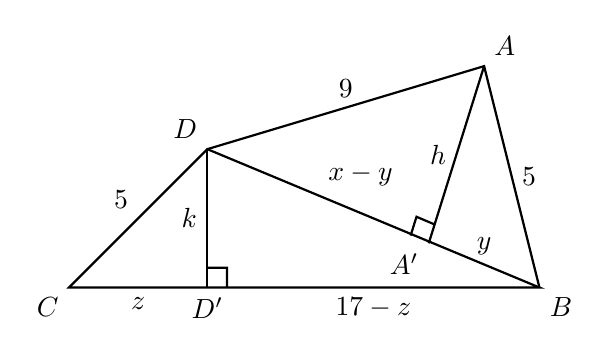
\begin{tikzpicture}[x=10,y=10, thick]
  \coordinate (C)  at (0,0);
  \coordinate (B)  at (17,0);
  \coordinate (D)  at (5,5);
  \coordinate (A)  at (15,8);
  \coordinate (D1) at (5,0);
  \coordinate (A1) at (13,1.6);
  \draw (C) node[below left] {$C$} -- (B) node[below right] {$B$} -- (D) node[above left] {$D$} -- cycle; 
  \draw (D) -- (A)  node[above right] {$A$} -- (B);
  \draw (D) -- (D1) node[below] {$D^{\prime}$};
  \draw (A) -- (A1) node[below left] {$A^{\prime}$};
  % label lengths
  \path (A) -- (B)  node[midway, right] {$5$};
  \path (A) -- (D)  node[midway, above] {$9$};
  \path (C) -- (D)  node[midway, above left] {$5$};
  \path (D) -- (D1) node[midway, left] {$k$};
  \path (C) -- (D1) node[midway, below] {$z$};
  \path (D1) -- (B) node[midway, below] {$17-z$};
  \path (B) -- (A1) node[midway, above] {$y$};
  \path (D) -- (A1) node[midway, above right] {$x-y$};
  \path (A) -- (A1) node[midway, left] {$h$};
  % mark angles
  \MarkRightAngle{A}{A1}{D}
  \MarkRightAngle{D}{D1}{B}
\end{tikzpicture}

\end{document}